\appendix
\section{Standard di riferimento}
\subsection{Standard ISO/IEC\textsubscript{G} 12207}
\subsubsection{Scopo}
La norma ha lo scopo principale di definire una struttura comune in modo che i professionisti coinvolti nello sviluppo del software (committenti, fornitori, sviluppatori, manutentori, operatori, manager e tecnici) possano utilizzare un linguaggio comune. Tale linguaggio è basato su una struttura di processi, attività, compiti e risultati prodotti. Il modello è flessibile e modulare in modo che ciascuno possa personalizzarlo a seconda delle proprie esigenze organizzative dei singoli progetti software.
Lo standard stabilisce i processi presenti nel ciclo di vita del software e, per ciascuno di essi, le attività da svolgere e i risultati da produrre.
\subsubsection{Tipi di Processo}
I processi sono suddivisi dalla norma in tre categorie:
\begin{itemize}
	\item \textbf{Processi primari}: I quali comprendono le attività direttamente legate allo sviluppo del software;
	\item \textbf{Processi di supporto}: I quali includono la gestione dei documenti e dei processi di controllo della qualità;
	\item \textbf{Processi organizzativi}: I quali coprono gli aspetti manageriali e di gestione delle risorse.
\end{itemize}
Per ciascun processo la norma evidenzia chiaramente:
\begin{itemize}
	\item \textbf{Obiettivo};
	\item \textbf{Responsabilità};
	\item \textbf{Lista delle attività che lo compongono};
	\item \textbf{Singoli compiti nei quali è suddivisa ogni attività}.
\end{itemize}
\begin{figure}[!ht]
	\centering
	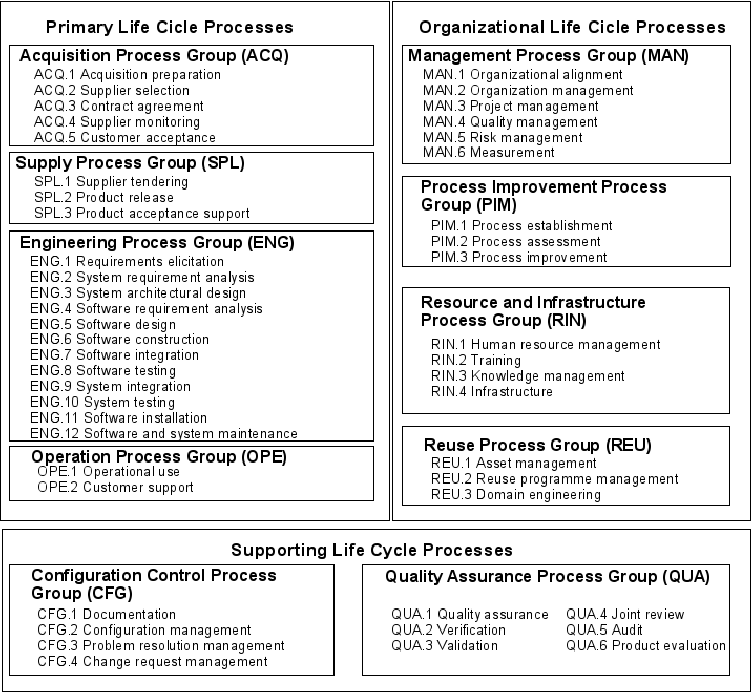
\includegraphics[scale=0.55]{img/ISO-IEC-12207-Processes.png}
	\caption{Processi definiti dallo standard ISO-IEC-12207}
\end{figure}
\newpage
\subsection{Standard ISO/IEC\textsubscript{G} 15504 SPICE}
\subsubsection{Scopo}
Lo standard ISO/IEC\textsubscript{G} 15504, chiamato anche SPICE (Software Process Improvement and Capability Determination), fornisce un framework\textsubscript{G} per la valutazione dei processi di un'organizzazione. Questo framework\textsubscript{G} può essere utilizzato dalle organizzazioni coinvolte nella pianificazione, gestione, monitoraggio, controllo e miglioramento di acquisizione, consegna, sviluppo, implementazione, evoluzione e manutenzione di prodotti e servizi di supporto.
\paragraph {Dimensione del processo}\mbox{}\\
La dimensione di processo del modello comprende 5 categorie di processi, rispettivamente composte da 4 a 10 processi:
\begin{itemize}
	\item \textbf{Cliente-fornitore}: Raggruppa i processi messi in atto da un acquirente per identificare il suo bisogno, selezionare il suo fornitore e ricevere la fornitura. Dal punto di vista del fornitore, questa categoria comprende le attività necessarie per la fornitura, la messa in servizio, il funzionamento e il supporto dell'utente;
	\item \textbf{Engineering}: Rientrano in questa categoria le attività di sviluppo software, nell'ambito del proprio ambiente di sistema, dalla fase di definizione alla fase di manutenzione;
	\item \textbf{Supporto}: Raggruppa i processi che consentono l'implementazione nell'ambito di un altro processo come la documentazione o i processi di gestione della configurazione;
	\item \textbf{Gestione}: Questa categoria contiene i processi caratteristici delle attività di gestione, in particolare la gestione dei progetti e le attività di gestione della qualità e  del rischio;
	\item \textbf{Organizzazione}: Questa categoria contiene i processi che riguardano l'intera organizzazione e non più il livello del singolo progetto.
\end{itemize}
\paragraph {Livelli di capacità e attributi di processo}\mbox{}\\
Il livello di capacità della dimensione è stabilito dai seguenti 6 gradi:
\begin{itemize}
	\item \textbf{Livello 0}: Processo incompleto o non eseguito,  non raggiunge i suoi obiettivi;
	\item \textbf{Livello 1}: Processo svolto e implementato, gli obiettivi sono raggiunti ma non viene verificato;
	\item \textbf{Livello 2}: Processo gestito, la sua attuazione è pianificata, monitorata e adattata;
	\item \textbf{Livello 3}: Processo consolidato, si basa su pratiche documentate ed è in grado di raggiungere i propri obiettivi;
	\item \textbf{Livello 4}: Processo prevedibile e ripetibile, la sua attuazione è condizionata da obiettivi di performance definiti;
	\item \textbf{Livello 5}: Processo di ottimizzazione, per raggiungere gli obiettivi attuali e futuri, è costantemente migliorato.
\end{itemize}
La capacità di processo viene misurata utilizzando gli attributi di processo. Lo standard identifica nove attributi di processo:
\begin{itemize}
	\item \textbf{1.1 - Prestazioni del processo};
	\item \textbf{2.1 - Gestione delle prestazioni};
	\item \textbf{2.2 - Gestione del prodotto di lavoro};
	\item \textbf{3.1 - Definizione del processo};
	\item \textbf{3.2 - Implementazione dei processi};
	\item \textbf{4.1 - Misura di processo};
	\item \textbf{4.2 - Controllo di processo};
	\item \textbf{5.1 - Innovazione di processo};
	\item \textbf{5.2 - Ottimizzazione del processo}.
\end{itemize}
In tutti i processi analizzati, vengono identificati una serie di forze e debolezze da cui si possono identificare potenziali di miglioramento. Le descrizioni del livello di maturità successivo mostrano le possibilità di miglioramento del processo. Questo standard richiede l'istituzione di una scala di valutazione. Gli attributi di ciascun processo sono valutati su una scala di valutazione suddivisa in quattro punti. I valori delle dimensioni dipendono dalla percentuale di raggiungimento degli attributi:
\begin{itemize}
	\item \textbf{N}: Non implementato (0-15\%);
	\item \textbf{P}: parzialmente implementato (> 15-50\%);
	\item \textbf{L}: Ampiamente implementato (> 50-85\%);
	\item \textbf{F}: completamente implementato (> 85\%).
\end{itemize}
\subsection{Standard ISO/IEC\textsubscript{G} 25000 SQuaRE}
\subsubsection{Scopo}
L'ISO/IEC\textsubscript{G} 25000 vuole dare un contributo alla sicurezza, alla funzionalità e manutenibilità del prodotto software, all'accuratezza dei dati, al raggiungimento della soddisfazione dell'utente in un'ottica preventiva e di qualità misurabile. Esso propone quindi modelli di qualità di riferimento a priori rispetto a quelli dei sistemi basati solo sulla difettosità a posteriori o monitorata durante le fasi del ciclo di vita del prodotto.
\subsubsection{ISO/IEC\textsubscript{G} 25010}
Uno standard molto rilevante della serie 25000 SQuaRE e l'ISO/IEC\textsubscript{G} 25010 il quale si occupa di definire gli obiettivi di qualità che deve avere un prodotto software.
Lo standard definisce quindi i termini di:
\begin{itemize}
	\item \textbf{Qualità interna}: La quale è riferita alle proprietà statiche e strutturali del software;
	\item \textbf{Qualità esterna}: La quale è riferita alle proprietà dinamiche e comportamentali del software;
	\item \textbf{Qualità in uso}: La quale è riferita al comportamento del software in un ambiente di utilizzo reale e alle varie interazioni con gli utenti.
\end{itemize}
\paragraph {Qualità interna ed esterna}\mbox{}\\
I modelli di qualità interna ed esterna comprendono 8 caratteristiche a loro volta sotto-categorizzate:
\begin{itemize}
	\item \textbf{Idoneità funzionale}: Suddivisa in:
	\begin{itemize}
		\item \textbf{Completezza};
		\item \textbf{Adeguatezza};
		\item \textbf{Correttezza}.
	\end{itemize}
	\item \textbf{Prestazione ed efficienza}: Suddivisa in:
	\begin{itemize}
		\item \textbf{Tempo};
		\item \textbf{Risorse};
		\item \textbf{Capacità}.
	\end{itemize}
	\item \textbf{Usabilità}: Suddivisa in:
	\begin{itemize}
		\item \textbf{Riconoscibilità};
		\item \textbf{Apprendibilità};
		\item \textbf{Operabilità};
		\item \textbf{Protezione errori};
		\item \textbf{Esteticità};
		\item \textbf{Accessibilità}.
	\end{itemize}
	\item \textbf{Affidabilità}: Suddivisa in:
	\begin{itemize}
		\item \textbf{Maturità};
		\item \textbf{Disponibilità};
		\item \textbf{Tolleranza};
		\item \textbf{Recuperabilità}.
	\end{itemize}
	\item \textbf{Sicurezza}: Suddivisa in:
	\begin{itemize}
		\item \textbf{Riservatezza};
		\item \textbf{Integrità};
		\item \textbf{Non ripudio};
		\item \textbf{Autenticazione};
		\item \textbf{Autenticità}.
	\end{itemize}
	\item \textbf{Manutenibilità}: Suddivisa in:
	\begin{itemize}
		\item \textbf{Modularità};
		\item \textbf{Riusabilità};
		\item \textbf{Analizzabilità};
		\item \textbf{Modificabilità};
		\item \textbf{Testabilità}.
	\end{itemize}
	\item \textbf{Compatibilità}: Suddivisa in:
	\begin{itemize}
		\item \textbf{Coesistenza};
		\item \textbf{Interoperabilità}.
	\end{itemize}
	\item \textbf{Portabilità}: Suddivisa in:
	\begin{itemize}
		\item \textbf{Adattabilità};
		\item \textbf{Installabilità};
		\item \textbf{Sostituibilità}.
	\end{itemize}
\end{itemize}
\paragraph {Qualità in uso del prodotto}\mbox{}\\
I modelli di qualità in uso del prodotto comprendono 5 caratteristiche a loro volta sotto-categorizzate:
\begin{itemize}
	\item \textbf{Efficacia};
	\item \textbf{Efficienza};
	\item \textbf{Soddisfazione};
	Suddivisa in:
	\begin{itemize}
		\item \textbf{Utilità};
		\item \textbf{Fiducia};
		\item \textbf{Piacere};
		\item \textbf{Comodità}.
	\end{itemize}
	\item \textbf{Assenza e attenuazione dei rischi}: Suddivisa in:
	\begin{itemize}
		\item \textbf{Economicità};
		\item \textbf{Salute};
		\item \textbf{Ambiente}.
	\end{itemize}
	\item \textbf{Copertura del contesto}: Suddivisa in:
	\begin{itemize}
		\item \textbf{Completezza};
		\item \textbf{Flessibilità}.
	\end{itemize}
\end{itemize}
\subsubsection{ISO/IEC\textsubscript{G} 25023}
Ad accompagnare lo standard 25010 troviamo lo standard 25023, il quale fornisce delle metriche di riferimento ai vari obiettivi di qualità di prodotto presenti nello standard a cui riferisce.





